\documentclass{beamer}
\usepackage{tikz,amsmath,hyperref,graphicx,stackrel,animate}
\usetikzlibrary{positioning,shadows,arrows,shapes,calc}
\newcommand{\argmax}{\operatornamewithlimits{argmax}}
\newcommand{\argmin}{\operatornamewithlimits{argmin}}
\mode<presentation>{\usetheme{Frankfurt}}
\AtBeginSection[]
{
  \begin{frame}<beamer>
    \frametitle{Outline}
    \tableofcontents[currentsection,currentsubsection]
  \end{frame}
}
\title{Lecture 5: Frequency}
\author{Mark Hasegawa-Johnson}
\date{ECE 417: Multimedia Signal Processing, Fall 2020}  
\begin{document}

% Title
\begin{frame}
  \maketitle
\end{frame}

% Title
\begin{frame}
  \tableofcontents
\end{frame}

%%%%%%%%%%%%%%%%%%%%%%%%%%%%%%%%%%%%%%%%%%%%
\section[Review]{Review: Equivalent Rectangular Bandwidth}
\setcounter{subsection}{1}

\begin{frame}
  \frametitle{Fletcher's Model of Masking, Reviewed}

  \begin{enumerate}
  \item The human ear pre-processes  the audio using a bank of bandpass filters.
  \item The power of the noise signal, in the  filter centered at $f_c$, is
    \[
    N_{f_c}=2\int_{0}^{F_S/2} R(f) |H_{f_c}(f)|^2 df
    \]
  \item The power of the tone is $T_{f_c}=A^2/2$, if the tone is at frequency $f_c$.
  \item If there is any band in which
    \[
    10\log_{10}\left(\frac{N_{f_c}+T_{f_c}}{N_{f_c}}\right)>1\mbox{dB}
    \]
    then the tone is audible.  Otherwise, not.
  \end{enumerate}
\end{frame}

\begin{frame}
  \frametitle{Equivalent rectangular bandwidth (ERB)}

  The frequency resolution of your ear is better at low frequencies.
  In fact, the dependence is roughly linear (Glasberg and Moore,
  1990):
  \[
  b \approx 0.108 f + 24.7
  \]
  These are often called (approximately) constant-Q filters, because
  the quality factor is
  \[
  Q = \frac{f}{b} \approx 9.26
  \]
  The dependence of $b$ on $f$ is not quite linear.  A more precise
  formula is given in (Moore and Glasberg, 1983) as:
  \[
  b = 6.23\left(\frac{f}{1000}\right)^2 + 93.39\left(\frac{f}{1000}\right)+28.52
  \]
\end{frame}

\begin{frame}
  \frametitle{Equivalent rectangular bandwidth (ERB)}

  \centerline{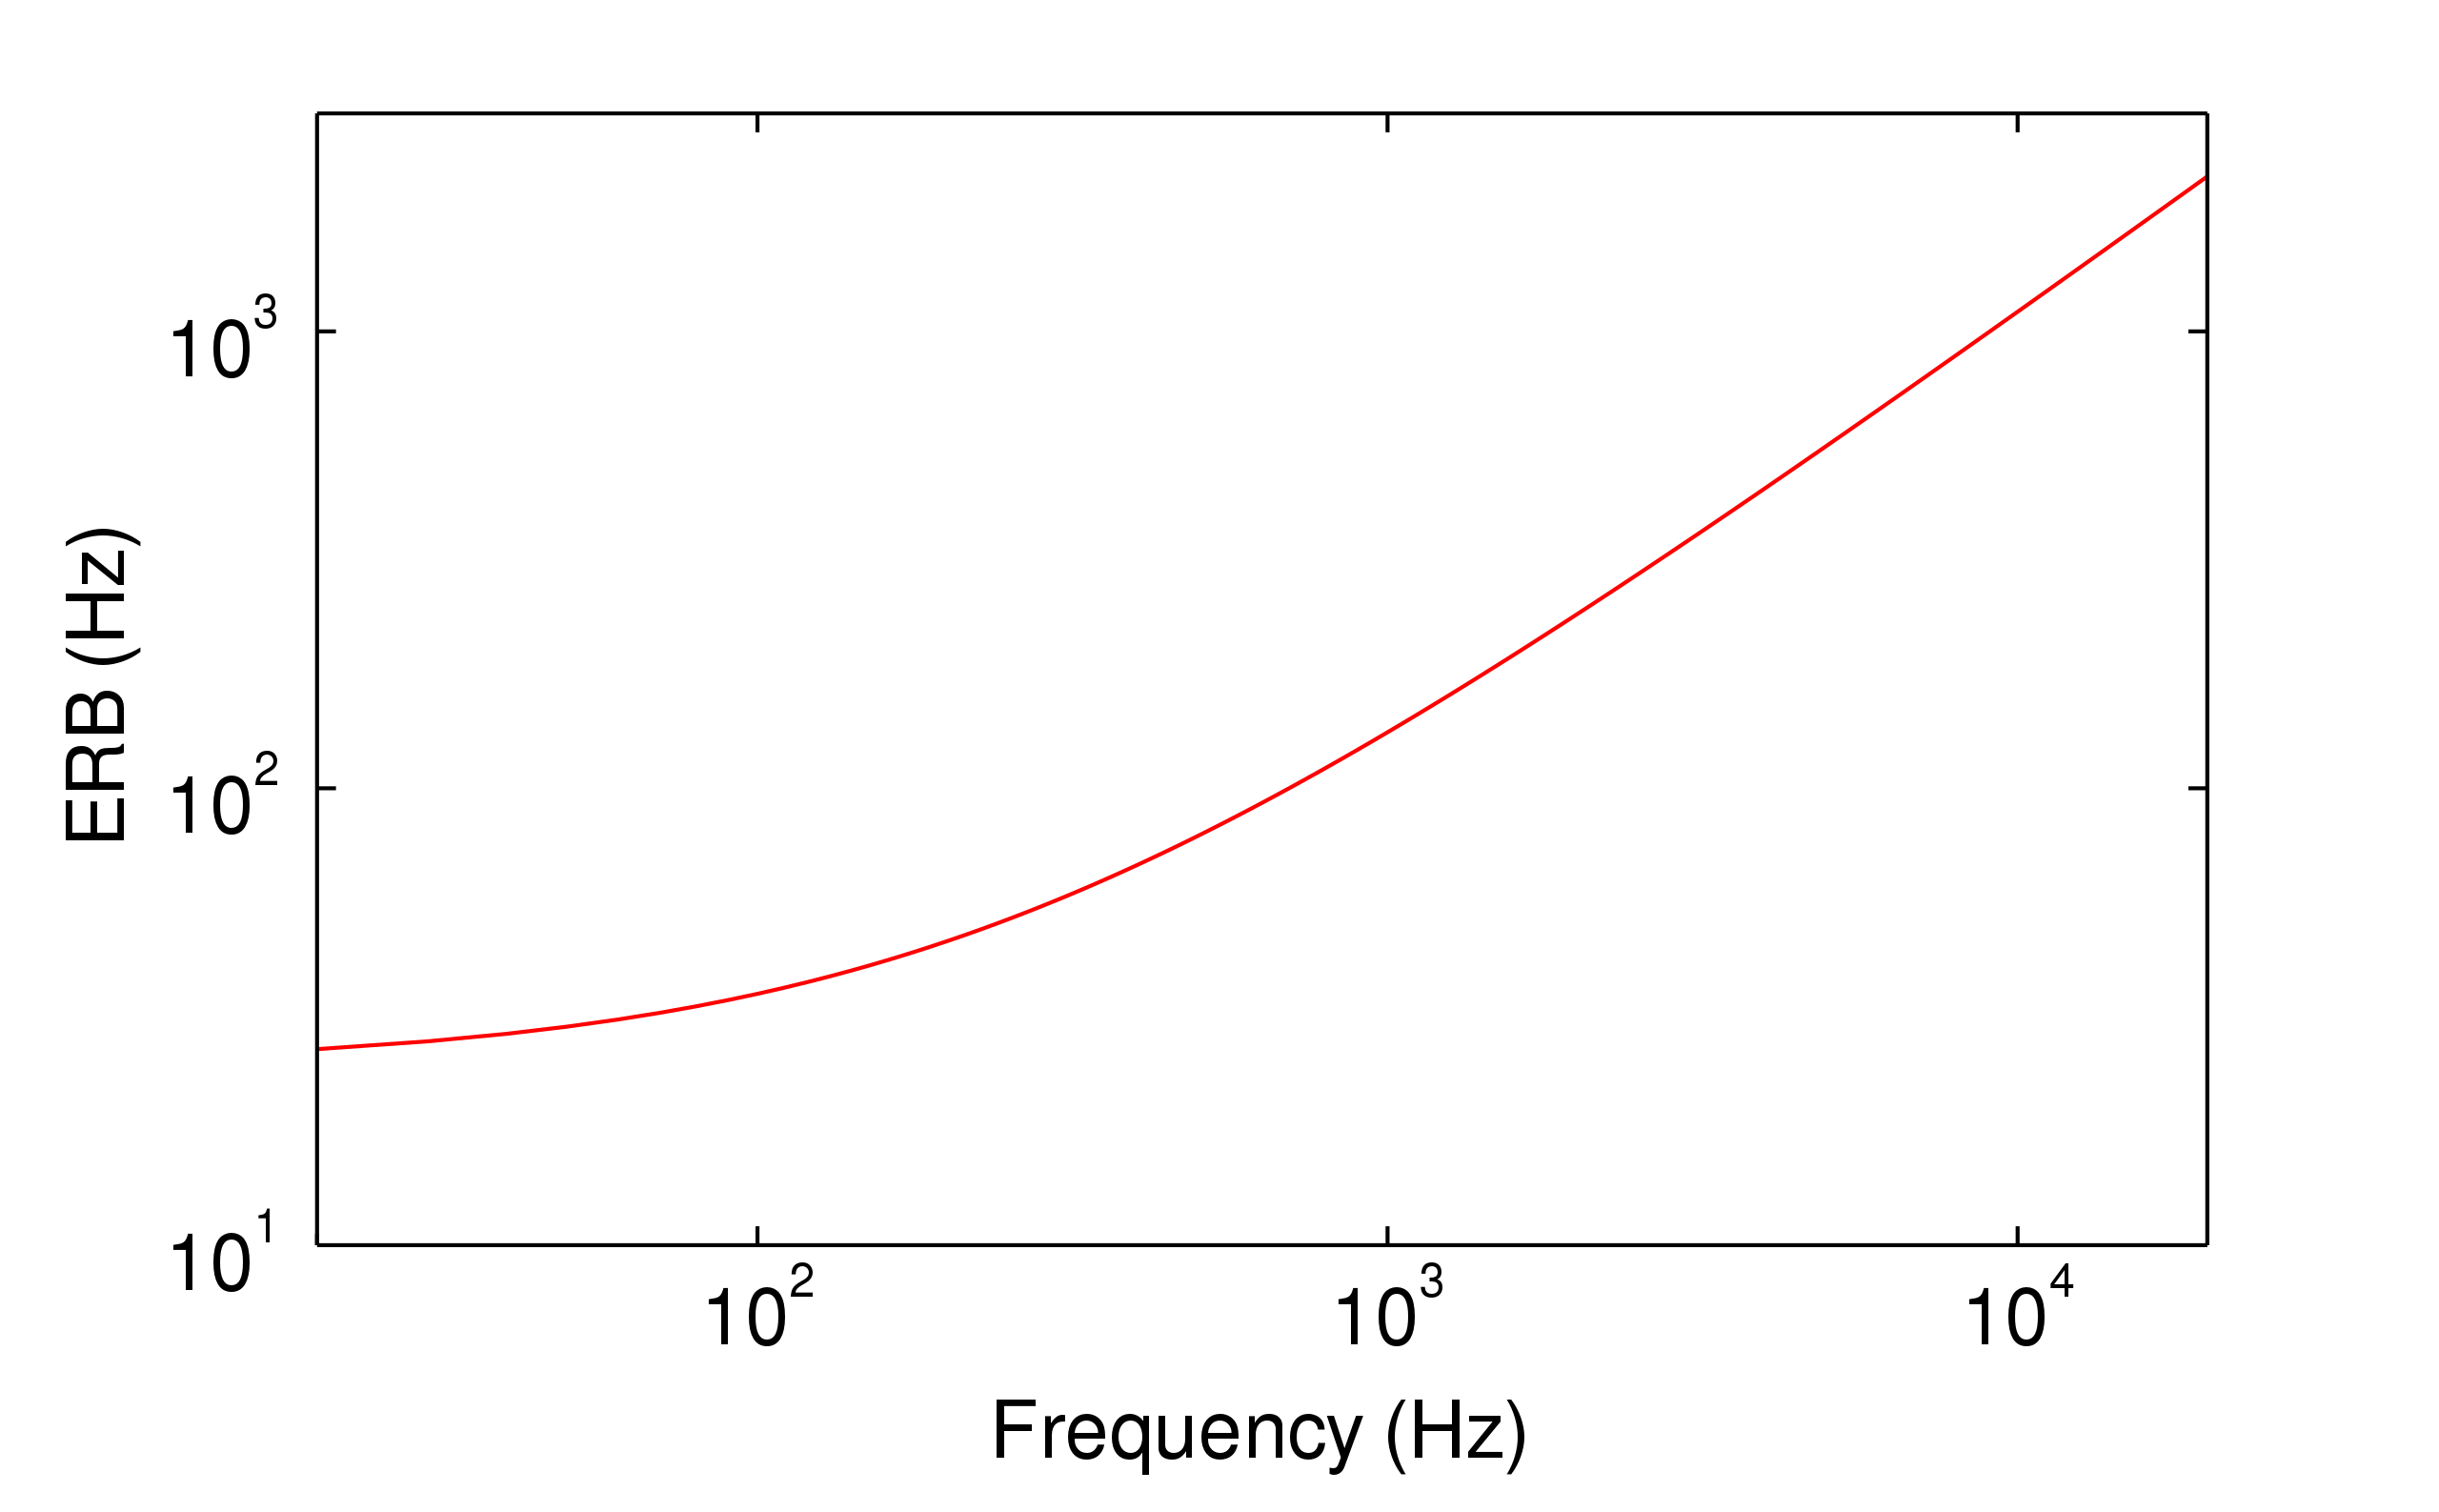
\includegraphics[height=2in]{../lec04/2560px-ERB_vs_frequency.png}}
  \begin{tiny}
    By Dick Lyon, public domain image 2009,
    \url{https://commons.wikimedia.org/wiki/File:ERB_vs_frequency.svg}
  \end{tiny}
\end{frame}

\begin{frame}
  \frametitle{The Gammatone Filter}

  The shape of the filter is not actually rectangular.  Patterson showed that it is
  \[
  |H(f)|^2 = \frac{1}{(b^2+(f-f_0)^2)^4}
  \]  
  He suggested modeling it as
  \[
  H(f) = \left(\frac{1}{b + j(f-f_0)}\right)^n + \left(\frac{1}{b + j(f+f_0)}\right)^n
  \]
  Whose inverse transform is a filter called a {\bf gammatone filter}.
  \[
  h(t) \propto t^{n-1} e^{-2\pi bt}\cos(2\pi f_0 t)u(t)
  \]
\end{frame}

\begin{frame}
  \frametitle{The Gammatone Filter: Spectrum}

  The top frame is a white noise, $x[n]$.  The middle frame is a
  gammatone filter at $f_c=1000$Hz, with a bandwidth of $b=128$Hz.
  The bottom frame is the filtered noise $y[n]$.

  \centerline{\includegraphics[height=2in]{../lec03/exp/gtfiltered_white_spectrum.png}}
\end{frame}
  
\begin{frame}
  \frametitle{The Gammatone Filter: Impulse Response}

  The top frame is a white noise, $x[n]$.  The middle frame is a
  gammatone filter at $f_c=1000$Hz, with a bandwidth of $b=128$Hz.
  The bottom frame is the filtered noise $y[n]$.

  \centerline{\includegraphics[height=2in]{../lec03/exp/gtfiltered_white_waveform.png}}
\end{frame}

\begin{frame}
  \frametitle{Frequency responses of the auditory filters}

  Here are the squared magnitude frequency responses ($|H(\omega)|^2$)
  of 26 of the 30000 auditory filters. I plotted these using the
  parametric model published by Patterson in 1974:
  \centerline{\includegraphics[height=2in]{../lec03/exp/gammatone_filterbank.png}}
\end{frame}

\begin{frame}
  \frametitle{Implications for Speech and Audio Recognition}

  \begin{itemize}
  \item Different human words must be audibly different.
  \item If a human being can't hear the difference, then they can't be different words.
  \item If humans can't hear small differences at high frequencies, then those differences
    can't possibly change the meaning of a word.
  \item For speech recognition, we should represent the low-frequency
    spectrum as precisely as the human ear represents it, and the
    high-frequency spectrum as imprecisely as the human ear represents
    it.
  \end{itemize}
\end{frame}

%%%%%%%%%%%%%%%%%%%%%%%%%%%%%%%%%%%%%%%%%%%%
\section[STFT]{Short-Time Fourier Transform}
\setcounter{subsection}{1}

%%%%%%%%%%%%%%%%%%%%%%%%%%%%%%%%%%%%%%%%%%%%
\section[Linear Frequency]{STFT as a Linear-Frequency Filterbank}
\setcounter{subsection}{1}

%%%%%%%%%%%%%%%%%%%%%%%%%%%%%%%%%%%%%%%%%%%%
\section[Nonlinear Frequency]{Implementing Nonlinear-Frequency Filterbanks Using the STFT}
\setcounter{subsection}{1}

%%%%%%%%%%%%%%%%%%%%%%%%%%%%%%%%%%%%%%%%%%%%
\section[Semitones]{Musical Pitch: Semitones, and Constant-Q Filterbanks}
\setcounter{subsection}{1}

\begin{frame}
  \frametitle{Musical Pitch}
  \centerline{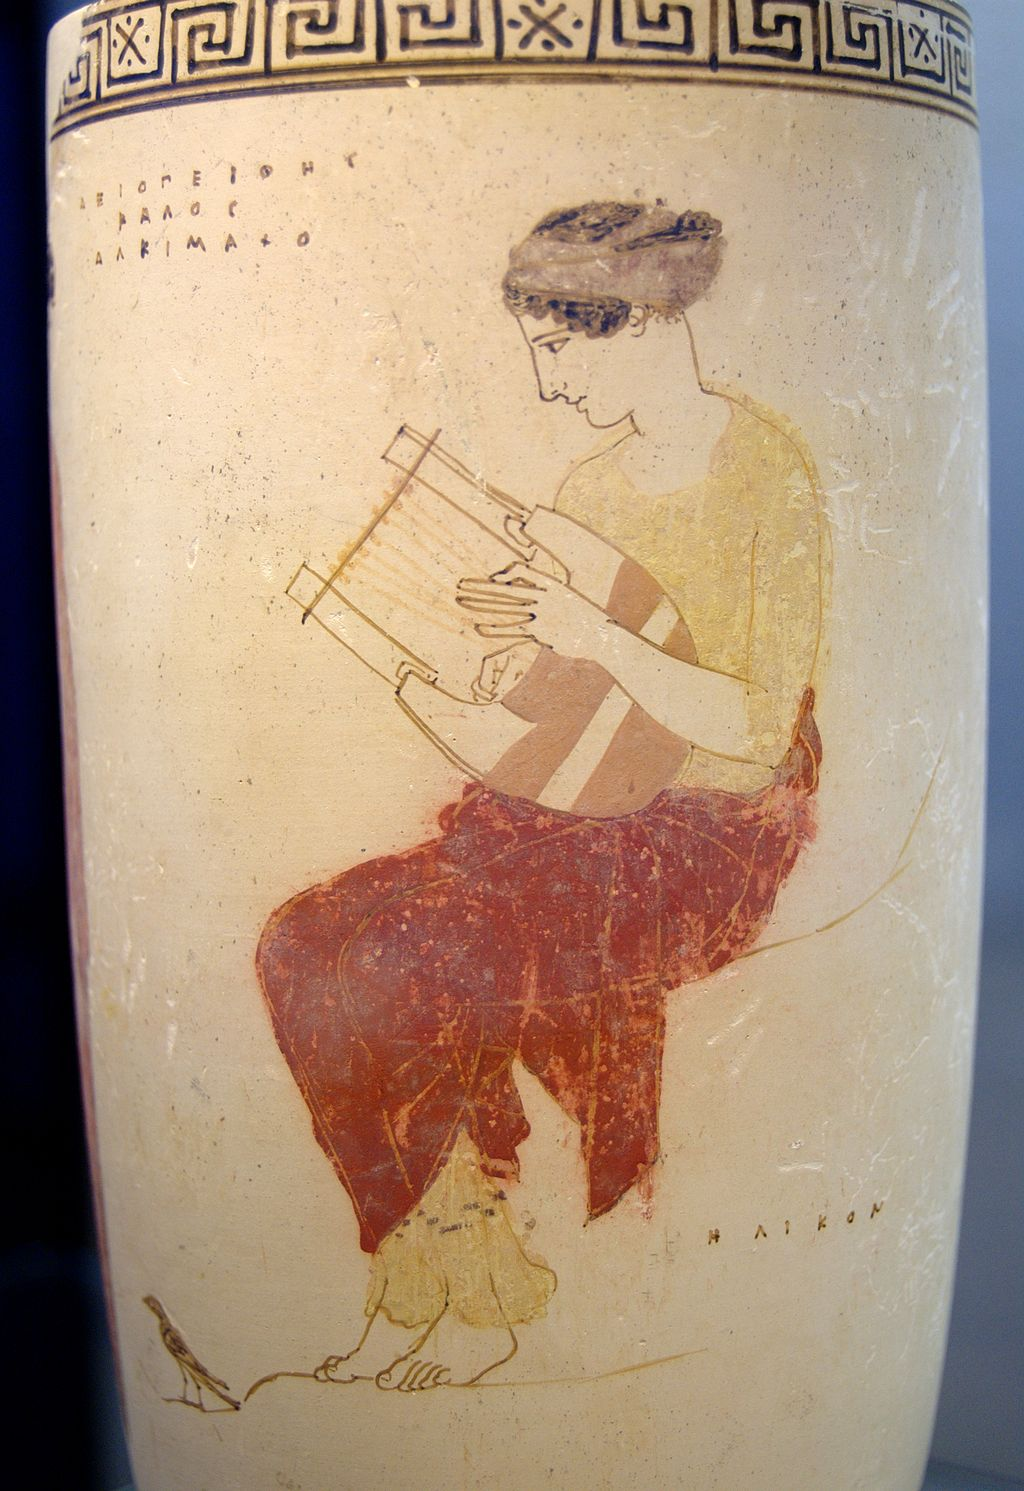
\includegraphics[height=2.5in]{helikon.jpg}}
  \begin{tiny}
    Muse playing the lyre, by the Achilles Painter.  Staatliche
    Antikensammlungen, public domain image by Bibi Saint-Pol,
    \url{https://commons.wikimedia.org/wiki/File:Mousai_Helikon_Staatliche_Antikensammlungen_Schoen80_n1.jpg}
  \end{tiny}
\end{frame}

\begin{frame}
  \frametitle{Pythagorean Tuning}
  \begin{itemize}
  \item Humans have always known that $f_2=2f_1$ (length of one string
    is twice the length of the other) means they are an octave apart
    (``same note'').
  \item A 3:2 ratio ($f_2=1.5f_1$) is a musical perfect fifth.
  \item Pythagoras is attributed with a system of tuning that created
    an 8-note scale by combining 3:2 and 2:1 ratios (``Pythagorean
    tuning''), used in some places until 1600.
  \end{itemize}
\end{frame}

\begin{frame}
  \frametitle{Pythagorean Tuning}
  \centerline{\fbox{\href{https://en.wikipedia.org/wiki/Pythagorean_tuning}{Pythagorean, Equal-Tempered, and Just Intonation}}}
\end{frame}

\begin{frame}
  \frametitle{Equal-Tempered Tuning}

  Equal-tempered tuning divides the octave into twelve equal ratios.
  \begin{itemize}
  \item {\bf Semitones:} the number of semitones, $s$, separating two
    tones $f_2$ and $f_1$ is given by
    \[
    s = 12\log_2\left(\frac{f_2}{f_1}\right)
    \]
  \item {\bf Cents:} the number of cents, $n$, separating two tones
    $f_2$ and $f_1$ is given by
    \[
    n = 1200\log_2\left(\frac{f_2}{f_1}\right)
    \]
  \end{itemize}
\end{frame}

\begin{frame}
  \frametitle{Constant-Q transform}

  STFT is
  \[
  X[k,m] = \sum_{n=0}^{N-1} w[n-m]x[n]e^{-j2\pi kn/N}
  \]
  \[
  f_k = \frac{kF_s}{N},~~~\omega_k =\frac{2\pi k}{N}
  \]
  \[
  Q = \frac{f_k}{b}
  \]
  \[
  N[k] = \frac{F_s}{f_k}Q
  \]
  Hamming window of length $N[k]$:
  \[
  w[k,n] = 0.54-0.46\cos\left(\frac{2\pi n}{N[k]-1}\right)
  \]
  $k^{\textrm{th}}$ frequency bin is located at:
  \[
  \omega_k = \frac{2\pi k}{N} = \frac{2\pi Q}{N[k]}
  \]
  The relative power of each bin will decrease at higher frequencies,
  as these sum over fewer terms. To compensate for this, we normalize
  by $N[k]$. After these modifications, we are left with
  \[
  X[k,m] = \frac{1}{N[k]}\sum_{n=0}^{N[k]-1} w[n-m]x[n]e^{-j2\pi kn/N}
  = \frac{1}{N[k]}\sum_{n=0}^{N[k]-1} w[n-m]x[n]e^{-j2\pi Qn/N[k]}
  \]
\end{frame}

%%%%%%%%%%%%%%%%%%%%%%%%%%%%%%%%%%%%%%%%%%%%
\section[Mel]{Perceived Pitch: Mels, and Mel-Filterbank Coefficients}
\setcounter{subsection}{1}

%%%%%%%%%%%%%%%%%%%%%%%%%%%%%%%%%%%%%%%%%%%%
\section[ERB]{Masking: Equivalent Rectangular Bandwidth Scale}
\setcounter{subsection}{1}

%%%%%%%%%%%%%%%%%%%%%%%%%%%%%%%%%%%%%%%%%%%%
\section[Summary]{Summary}
\setcounter{subsection}{1}



\end{document}

